\let\negmedspace\undefined
\let\negthickspace\undefined
\documentclass[journal,12pt,twocolumn]{IEEEtran}
\usepackage{cite}
\usepackage{amsmath,amssymb,amsfonts,amsthm}
\usepackage{algorithmic}
\usepackage{graphicx}
\usepackage{textcomp}
\usepackage{xcolor}
\usepackage{txfonts}
\usepackage{listings}
\usepackage{enumitem}
\usepackage{mathtools}
\usepackage{gensymb}
\usepackage{comment}
\usepackage[breaklinks=true]{hyperref}
\usepackage{tkz-euclide} 
\usepackage{listings}
\usepackage{gvv}                                        
\def\inputGnumericTable{}                                 
\usepackage[latin1]{inputenc}                                
\usepackage{color}                                            
\usepackage{array}                                            
\usepackage{longtable}                                       
\usepackage{calc}                                             
\usepackage{multirow}                                         
\usepackage{hhline}                                           
\usepackage{ifthen}                                           
\usepackage{lscape}

\newtheorem{theorem}{Theorem}[section]
\newtheorem{problem}{Problem}
\newtheorem{proposition}{Proposition}[section]
\newtheorem{lemma}{Lemma}[section]
\newtheorem{corollary}[theorem]{Corollary}
\newtheorem{example}{Example}[section]
\newtheorem{definition}[problem]{Definition}
\newcommand{\BEQA}{\begin{eqnarray}}
\newcommand{\EEQA}{\end{eqnarray}}
\newcommand{\define}{\stackrel{\triangle}{=}}
\theoremstyle{remark}
\newtheorem{rem}{Remark}
\begin{document}

\bibliographystyle{IEEEtran}
\vspace{3cm}

\title{11.9.5}
\author{EE23BTECH11029 - Kanishk}
\maketitle

\bigskip



\renewcommand{\thefigure}{\theenumi}
\renewcommand{\thetable}{\theenumi}
\textbf{Question}:\\ 
The sum of the first four terms of an A.P. is 56. The sum of the last four terms is
112. If its first term is 11, then find the number of terms.\\

\textbf{Solution}:\\ 

\footnotesize
\centering
\begin{tabular}{|c|c|c|}
\hline
Symbol & Value & Description\\
\hline
$S_1$ & $56$ & Sum of the first four terms of AP\\
\hline
$S_2$ & $112$& Sum of the last four terms of AP\\
\hline
$x(0)$ & $11$ & First term of AP \\
\hline
$d$ &$ 2$ & Common difference of AP\\
\hline
$n+1$ & $11$ & Number of terms of AP\\
\hline
$x(n)$ & $31$ & Last term of AP\\
\hline

\end{tabular}
\\
\small

\centering{Input Parameters}

\begin{align}
S_1&=\frac{4}{2}\brak{2x\brak{0}+3d}\\
\frac{4}{2}\brak{2x\brak{0}+3d}&=56\\
2x\brak{0}+3d&=28\\
d&=2
\end{align}

\begin{align}
S_2&=1\frac{4}{2}\brak{2x\brak{n}+3\brak{-d}}\\
\frac{4}{2}\brak{2x\brak{n}+3\brak{-d}}&=112\\
2x\brak{n}-3d&=56\\
x\brak{n}&=31\\
x\brak{0}+\brak{n}2&=31\\
n&=10
\end{align}
\newpage
\begin{figure}
    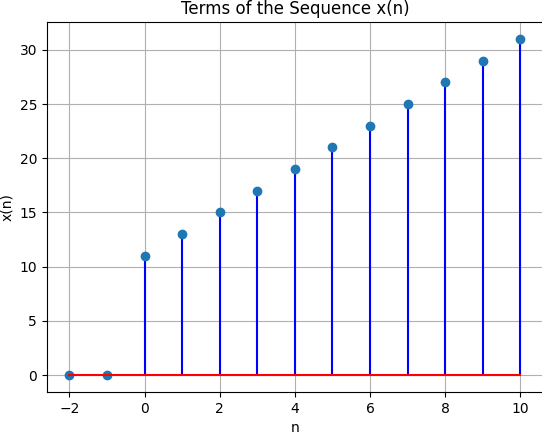
\includegraphics[width=\columnwidth]{fig.png}
    \centering
    Plot x(n) vs n
    \label{fig:enter-label}
\end{figure}

\begin{align}
	x \brak{n} &\system{Z} X \brak{z}\\
	x\brak{n}&=x\brak{0}+2n
\end{align}

\begin{align}
X\brak{z}&= \sum_{n=-\infty}^{\infty} x\brak{n}Z^{-n} \\
&=\sum_{n=0}^{\infty} x\brak{0}Z^{-n} + \sum_{n=-0}^{\infty}2nZ^{-n}\\
&=\frac{x\brak{0}}{1-Z^{-1}}+2\frac{Z^{-n}}{\brak{1-Z^{-1}}^{2}}, |Z|>1
\end{align}








\end{document}